\section{Large Language Diffusion Models (LLDMs)}
\begin{frame}{}
    \LARGE \textbf{Large Language Diffusion Models (LLDMs)}
\end{frame}

\begin{frame}[allowframebreaks]{LLDMs: Diffusion for Text Generation}
    \begin{figure}
        \centering
        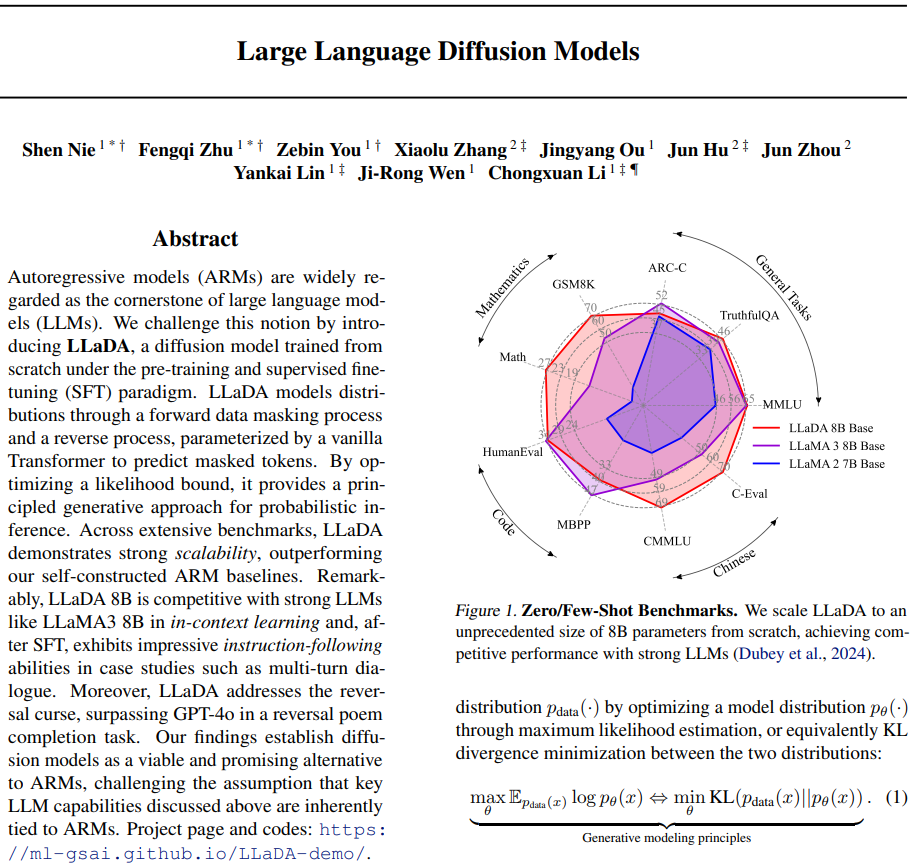
\includegraphics[height=0.80\textheight,width=\textwidth,keepaspectratio]{images/recent-advance/lldm-paper.png}
        \caption*{\scriptsize Source: Nie et al., ``Large Language Diffusion Models,'' NeurIPS 2025, \href{https://arxiv.org/abs/2502.09992v2}{arXiv:2502.09992v2}, first page.}
    \end{figure}
\framebreak
    \begin{itemize}
        \item \textbf{Emerging trend:} Use diffusion instead of autoregression for text generation
    \end{itemize}
    \vspace{0.5em}
    \textbf{Key Idea:} the model is a \textbf{mask predictor}, not a next-token predictor.
    \begin{itemize}
        \item A forward process corrupts text by replacing tokens with a mask symbol; the reverse process fills masks back in.
        \item The reverse process is a transformer \textbf{without a causal mask}, so every prediction is conditioned on the whole sequence in both directions.
        \item Generation starts from a fully masked answer and unmasks tokens over repeated passes, in whatever order the model is most confident about, rather than strictly left to right.
    \end{itemize}

\framebreak

    \textbf{LLaDA} (Nie et al., 2025) is the first such model built at LLM scale:
    \begin{itemize}
        \item 8B parameters, pre-trained from scratch on 2.3T tokens, then supervised fine-tuned on 4.5M prompt-response pairs, using the same recipe as an autoregressive LLM.
        \item Competitive with LLaMA 3 8B in in-context learning on 2.3T tokens against its 15T, and ahead of it on mathematics and Chinese benchmarks.
        \item Answers reversal questions that left-to-right models fail, beating GPT-4o at completing a poem backwards.
    \end{itemize}
\framebreak
    \textbf{Antecedents:}
    \begin{itemize}
        \item Diffusion-LM (Li et al., 2022): continuous diffusion over word-vector sequences, for controllable generation at small scale.
        \item Masked, or discrete, diffusion: the forward process replaces tokens with a mask symbol instead of adding Gaussian noise, which is what makes text diffusion tractable at scale.
    \end{itemize}
    \vspace{0.5em}
    \textbf{Note:} Still early work, but it shows that scale, in-context learning, and instruction following are not exclusive to left-to-right models
\framebreak
    \begin{figure}
        \centering
        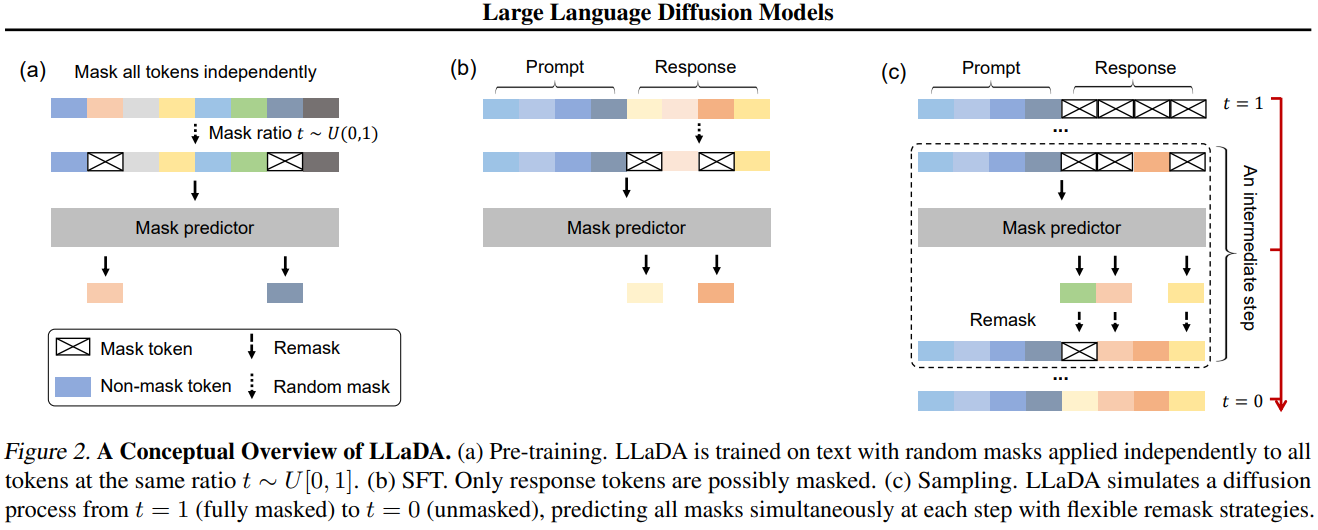
\includegraphics[height=0.72\textheight,width=\textwidth,keepaspectratio]{images/recent-advance/lldm-overview.png}
        \caption*{\scriptsize Source: Nie et al., NeurIPS 2025, \href{https://arxiv.org/abs/2502.09992v2}{arXiv:2502.09992v2}, Figure~2.}
    \end{figure}
\framebreak
    \begin{figure}
        \centering
        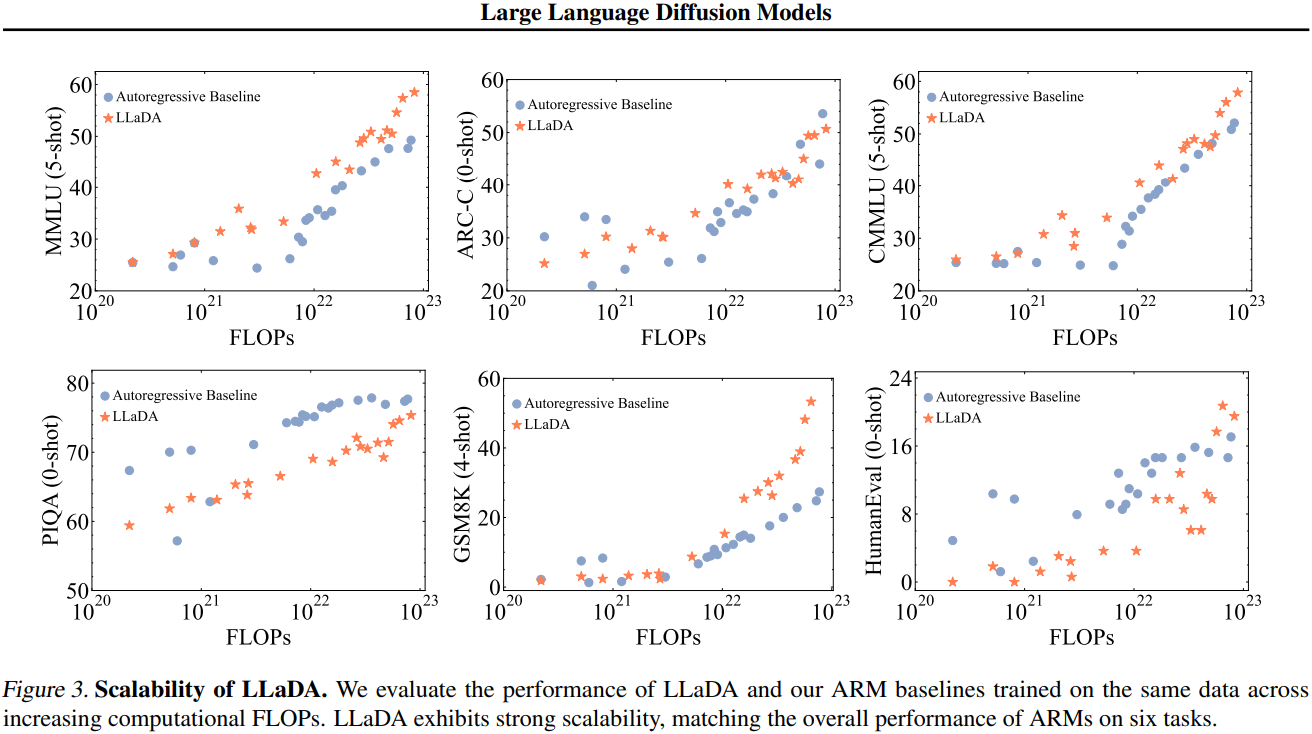
\includegraphics[height=0.74\textheight,width=\textwidth,keepaspectratio]{images/recent-advance/lldm-scalability.png}
        \caption*{\scriptsize Source: Nie et al., NeurIPS 2025, \href{https://arxiv.org/abs/2502.09992v2}{arXiv:2502.09992v2}, Figure~3.}
    \end{figure}

\framebreak
    \begin{figure}
        \centering
        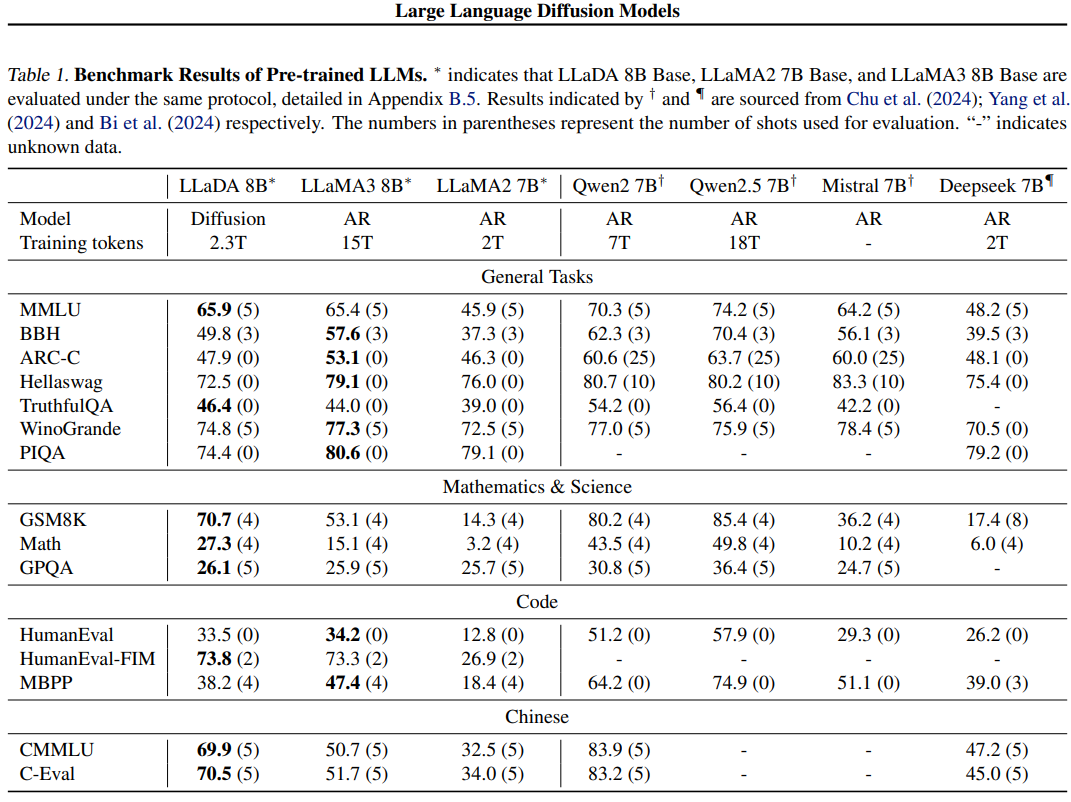
\includegraphics[height=0.78\textheight,width=\textwidth,keepaspectratio]{images/recent-advance/lldm-benchmark-result.png}
        \caption*{\scriptsize LLaDA 8B reaches this from 2.3T training tokens, against 15T for LLaMA 3 8B. Source: Nie et al., NeurIPS 2025, \href{https://arxiv.org/abs/2502.09992v2}{arXiv:2502.09992v2}, Table~1 (several values were revised in v3).}
    \end{figure}

\framebreak
    \begin{figure}
        \centering
        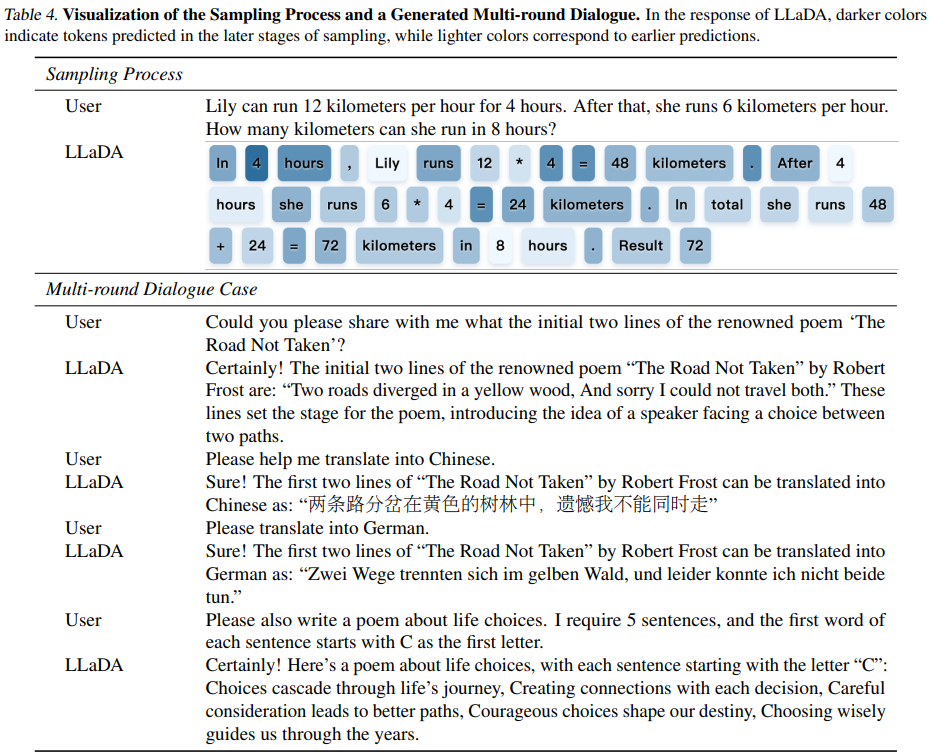
\includegraphics[height=0.76\textheight,width=\textwidth,keepaspectratio]{images/recent-advance/lldm-sampling.png}
        \caption*{\scriptsize Shading marks when each token was fixed: the answer does not fill in left to right. Source: Nie et al., NeurIPS 2025, \href{https://arxiv.org/abs/2502.09992v2}{arXiv:2502.09992v2}, Table~4 (Table~3 in v3).}
    \end{figure}
\end{frame}

\begin{frame}[allowframebreaks]{The Masking Process}
    \textbf{Forward process.} A time $t$ runs from 0, the intact sequence, to 1, a fully masked one. Draw $t \sim U(0,1)$ and replace each token independently with the mask symbol \texttt{M} with probability $t$.
    \vspace{0.5em}

    \textbf{Training.} The mask predictor $p_\theta$ sees the corrupted sequence $x_t$ and predicts every masked position at once. Only masked positions contribute to the loss, rescaled by $t$ so that heavily and lightly masked samples count equally:
    \begin{equation}
        \mathcal{L}(\theta) = -\frac{1}{tL} \sum_{i=1}^{L} \mathbf{1}[x_t^i = \texttt{M}] \, \log p_\theta(x_0^i \mid x_t)
    \end{equation}
    where $L$ is the sequence length. This is an upper bound on the negative log-likelihood, so training is still maximum likelihood, and the same objective is reused for supervised fine-tuning by masking only the response.

\framebreak

    \textbf{Sampling.} Choose an answer length $L$ and a number of steps $N$, and start from a fully masked answer. Each step moves from $t$ to $s = t - 1/N$:
    \begin{enumerate}
        \item Predict a token at every masked position.
        \item Remask some of those predictions, so that the number of revealed tokens grows on a fixed schedule as $s$ falls to 0.
    \end{enumerate}
    \vspace{0.5em}
    \textbf{Which ones to remask:}
    \begin{itemize}
        \item \textbf{Random remasking:} remask each fresh prediction with probability $s/t$.
        \item \textbf{Low-confidence remasking:} keep the predictions the model scores highest and remask the rest. This works better, and is why the sampling trace shown earlier fixes confident tokens first.
    \end{itemize}
    \vspace{0.5em}
    $N$ is the knob that trades quality against cost: an autoregressive model needs one pass per token, while a diffusion model needs one pass per step, whatever the answer length.
\end{frame}

\begin{frame}[allowframebreaks]{LLDMs: Algorithm Overview}
    \begin{figure}
        \centering
        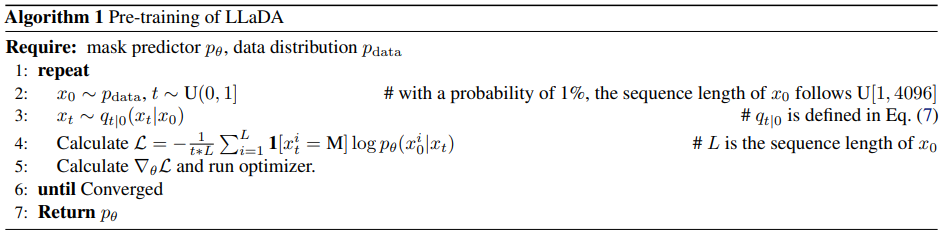
\includegraphics[height=0.66\textheight,width=\textwidth,keepaspectratio]{images/recent-advance/lldm-pretraining.png}
        \caption*{\scriptsize Pre-training. In 1\% of steps the sequence length is drawn from $U[1,4096]$ instead of the full 4096, so the model also sees short inputs. Source: Nie et al., NeurIPS 2025, \href{https://arxiv.org/abs/2502.09992v2}{arXiv:2502.09992v2}, Algorithm~1.}
    \end{figure}
\framebreak
    \begin{figure}
        \centering
        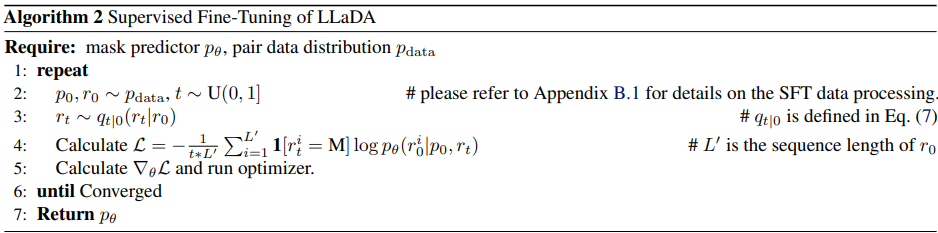
\includegraphics[height=0.66\textheight,width=\textwidth,keepaspectratio]{images/recent-advance/lldm-supervised-finetuning.png}
        \caption*{\scriptsize Fine-tuning. Only the response $r_0$ is masked; the prompt $p_0$ is always visible, so the same loss now trains a conditional model. Source: Nie et al., NeurIPS 2025, \href{https://arxiv.org/abs/2502.09992v2}{arXiv:2502.09992v2}, Algorithm~2.}
    \end{figure}
\framebreak
    \begin{figure}
        \centering
        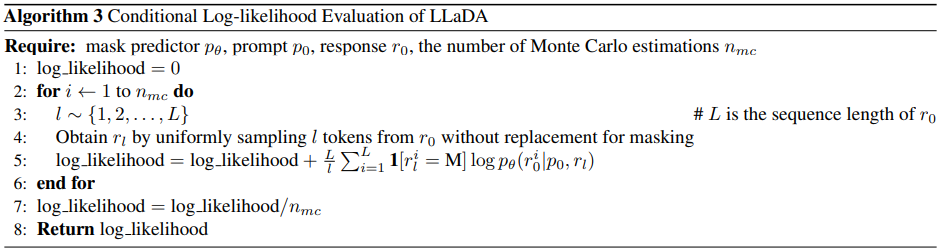
\includegraphics[height=0.66\textheight,width=\textwidth,keepaspectratio]{images/recent-advance/lldm-log-likelihood.png}
        \caption*{\scriptsize Evaluation. There is no chain rule to multiply out, so likelihood is estimated by Monte Carlo: mask $l$ random tokens, score them, and average over draws. Source: Nie et al., NeurIPS 2025, \href{https://arxiv.org/abs/2502.09992v2}{arXiv:2502.09992v2}, Algorithm~3.}
    \end{figure}
\end{frame}

\begin{frame}{What LLDMs Cost}
    \textbf{The reported gains come with open problems:}
    \begin{itemize}
        \item \textbf{Answer length is set in advance.} It is an input to sampling, not something the model decides, and an adaptive length is left to future work.
        \item \textbf{No inference machinery yet.} Bidirectional attention means there is no prefix to cache, so the KV-cache and the specialised attention and position schemes that autoregressive serving relies on do not carry over. The reported speed is not the point of the work.
        \item \textbf{Likelihoods are estimates.} Without a left-to-right factorization there is no exact sequence likelihood, only a Monte Carlo bound, which makes evaluation noisier.
        \item \textbf{Alignment stops at fine-tuning.} LLaDA has had no RL-based alignment, and it trails LLaMA 3 8B Instruct, which has.
        \item \textbf{The comparison is not fully controlled.} Compute limits kept the head-to-head against autoregressive baselines below $10^{23}$ FLOPs, so the largest models are compared across different training budgets.
    \end{itemize}
\end{frame}
